\clearpage
\section{Dense sampling and the second manuscript term}
\label{sec:dense-second-order}
The purpose of this scan is to distinguish an improved residual from
an improved estimate of a CFT coefficient. In particular, adding a
second basis function always reduces the training sum of squares, but
need not move the first coefficient towards its theoretical value.
We therefore compare $F_1$ and $F_2$ on exactly the same observations,
using the objective in Eq.~\eqref{eq:objective}, and examine both
coefficients rather than the residual alone.

\subsection{Additional geometries and direct coefficient comparisons}
Both CFTs first receive the same additional 47 even sizes between 60 and
6000. Start with $N_j=2\operatorname{round}[30\,100^{j/48}]$ for
$j=0,\ldots,48$, and omit sizes already present. Every new size uses
$\ell=6,7,8,9,10$ and computes both interval observables for all six
ordered pairs. A further 188 Ising sizes complete the progression
$N=200,204,\ldots,1000$, concentrating observations where the known
$x^6$ term is measurable. The two sets are defined in
Eq.~\eqref{eq:dense-grid}. No new size exceeds the existing maxima
8192 and 16384. The resulting 1175 Ising and 235 boson new geometries per direction fill
the intermediate fractions without changing any previously computed
entropy. The exact executed sizes, checks, and timings are retained
in \path{data/dense_grid_manifest.json} and the production CSVs.
The subsequent refinement in Appendix~\ref{sec:common-window-results}
adds 48 further sizes for each CFT while keeping all fitting windows
fixed. Every current fit, plotted coefficient and window-sensitivity
comparison below uses the combined data; the two grid manifests
distinguish the original dense scan from this later refinement.

Let $q=D^A$ with $z=x$ for a small interval, or
$q=\delta=\log 2-D^B$ with $z=y$ for its large complement. With the
pair-specific powers $r_0,r_1$ in Eq.~\eqref{eq:fit}, the two models are
$F_1=c_0z^{r_0}$ and $F_2=c_0z^{r_0}+c_1z^{r_1}$.
Both coefficients in $F_2$ are estimated; neither is fixed to theory.
All amplitudes include their powers of $\pi$.
For the leading discrepancy $\eta_c$ in Eq.~\eqref{eq:metrics}, define
\begin{equation}
 \Delta_0=|\eta_c(F_1)|-|\eta_c(F_2)|.
 \label{eq:dense-coefficient-gain}
\end{equation}
A positive $\Delta_0$, measured in percentage points, means that
including the second term improves the leading coefficient on that
window. This is distinct from the residual gain $G$ and the omitted-size
prediction gain $G_{\rm CV}$. All reported fits and omitted-size
training sets retain at least forty observations.

For the known Ising coefficients, the supplied manuscript gives
\begin{align}
 D^A_{I\mid\eps}&=\frac{2\pi^4}{15}x^4-\frac{8\pi^6}{45}x^6+O(x^8),\nonumber\\
 D^A_{\eps\mid I}&=\frac{2\pi^4}{15}x^4-\frac{8\pi^6}{21}x^6+O(x^8).
 \label{eq:dense-known-ising}
\end{align}
These are the $p=1/2$ specializations of the two Ising mixture
expressions in the supplied source~\cite{theoryLarge}. No missing
subleading coefficient is derived or assumed. The unknown analytical
cells remain blank.

\subsection{What is resolved by the dense scan}
The principal comparisons improve the absolute leading-coefficient discrepancy in 22 of the 24 ordered-pair/interval cases. Of these, 18 also improve the omitted-size prediction residual. Tables~\ref{tab:dense-small-ising}--\ref{tab:dense-large-boson-second} retain the failures as well as the improvements. A lower residual alone is therefore not counted as recovery of a CFT coefficient.

For boson large intervals, $00\mid ss$ on $W=(0,0.005]$ changes the leading discrepancy from $2.2645\%$ under $F_1$ to $2.3499\%$ under $F_2$. This is a failure to improve that coefficient, even if the residual decreases.

For boson large intervals, $ss\mid 00$ on $W=(0,0.005]$ changes the leading discrepancy from $2.2636\%$ under $F_1$ to $2.351\%$ under $F_2$. This is a failure to improve that coefficient, even if the residual decreases.

The adopted windows are Eq.~\eqref{eq:common-fit-windows}. The large-boson upper cutoff is prescribed as $0.005$: Appendix~\ref{sec:common-window-results} reports its neighboring-cutoff and omitted-size sensitivity. Improvement of a leading coefficient does not establish recovery of its unknown second coefficient.

For the two known Ising directions, the pooled window $W_x=(0,0.02]$ gives $c_1=-170.71$ and $-355.38$, respectively. Their signed discrepancies from Eq.~\eqref{eq:dense-known-ising} are $-0.12193\%$ and $-2.9657\%$. The leading coefficient improves in 2 of these two directions; the omitted-size ranges in Table~\ref{tab:dense-small-ising-second} expose the remaining sensitivity of the pooled second coefficients.

At $\ell=10$, the separate-length fits on $W_x=(0,0.006]$ contain 82 points each and give $c_1=-169.27$ and $-362.08$. Their discrepancies are $-0.96408\%$ and $-1.1357\%$. The leading coefficients differ from theory by about $0.49974\%$. The dependence on $\ell$ and on the upper endpoint is visible in Fig.~\ref{fig:dense-subsystem}; these small omitted-size ranges do not erase the finite-length offset.

The cutoff propagation in Eq.~\eqref{eq:dense-cutoff-bound} gives $b_1=0.0027612$ and $0.0027345$ for the same $\ell=10$ fits. The recorded cutoff variation is much smaller than the observed second-coefficient discrepancy. These values are sensitivity bounds for the tested cutoff variation only.

The separate shared-window diagnostic uses $W_x=W_y=(0,0.006]$ and improves the leading coefficient in 21 of 24 cases; see Fig.~\ref{fig:dense-shared}. Across all 744 common windows in the recorded scan on the current grid, the largest improvement count is 23 of 24. No single interval in that scan improves all pairs simultaneously. This does not preclude the four CFT/interval-specific common windows now adopted. In particular, one apparent near-match does not establish a universal interval where every second coefficient is resolved.

For example, that same shared window gives pooled Ising second coefficients $-1029.7$ and $-1220.3$. Their signed discrepancies from Eq.~\eqref{eq:dense-known-ising} are $502.46\%$ and $233.2\%$. An improved leading amplitude cannot by itself validate the second term. The unknown second coefficients in the tables are estimates of the specified finite-$\ell$ two-term fits, not established continuum constants.

The chosen windows were explored with these deterministic data, so
their agreement with theory is an exploratory comparison rather than
a blind prediction. Omitted-size refits test sensitivity to individual
chain sizes; they do not remove the effect of selecting a window.
The fitted $c_1$ should be interpreted as a coefficient of the specified
two-term truncation unless it remains stable as the window changes.
The separate-$\ell$ comparison uses exactly the same $F_2$ model on
$W_x=(0,0.006]$ for each of the five lengths. It estimates both
coefficients independently for each length and adds no new power.
Different finite-$\ell$ leading amplitudes can influence a pooled
second coefficient when their relative sampling changes across the
window. The separate-length results expose this directly; they are
not an extrapolation to $\ell\to\infty$.

We also propagate the recorded entropy variation under the support-cutoff
checks to the two fitted coefficients. For the design matrix
$X_{ij}=x_i^{r_j}$, let $P=(X^TX)^{-1}X^T$ and let $s_i$ be the
observed span of entropy values when the numerical support cutoff is
varied. The resulting sensitivity bound is
\begin{equation}
 b_j=\sum_i |P_{ji}|s_i.
 \label{eq:dense-cutoff-bound}
\end{equation}
This bounds coefficient changes if each data perturbation is no larger
than its recorded span. It is an empirical cutoff-sensitivity check,
not an error bound for the continuum approximation or for all
floating-point operations. The implementation uses scaled columns
and a pseudoinverse, avoiding the large dynamic range of the powers.

To expose the second term directly, plot
\begin{equation}
 U(z)=\frac{q(z)}{z^{r_0}},\qquad t=z^{r_1-r_0}.
 \label{eq:dense-normalized-curve}
\end{equation}
The plotted $F_2$ curve is then a straight line $U=c_0+c_1t$.
The fit is still performed in $q$, not in $U$; the transformation is
only a visualization. Separate symbols retain the subsystem length,
so disagreement between lengths is visible without introducing an
extra lattice-correction ansatz. At fixed $\ell$, increasing $N$
reduces $z$ but does not take a continuum limit with $\ell\to\infty$.
Consequently, denser sampling alone cannot guarantee exact recovery
of the continuum coefficients.

\begin{figure}[!htbp]\centering
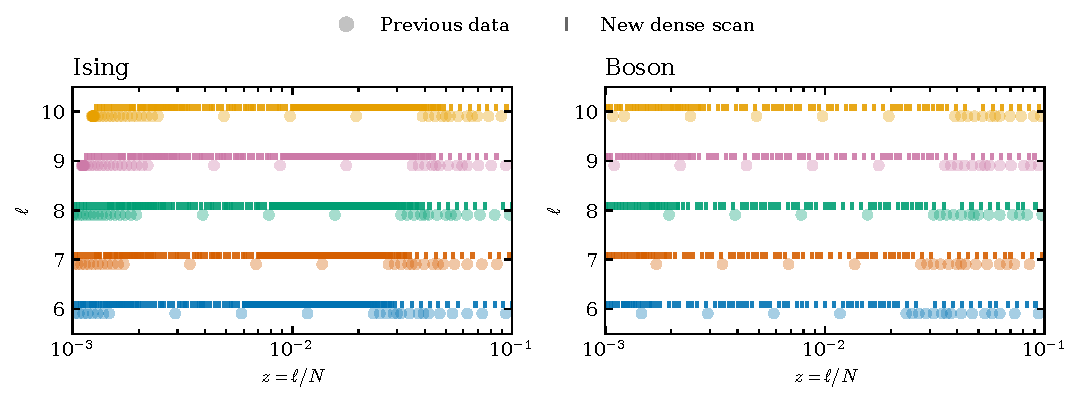
\includegraphics[width=.97\linewidth]{../figs/dense_sampling.pdf}
\caption{Sampling between $10^{-3}$ and $10^{-1}$, common to both interval observables. Circles are the geometries preceding the dense study; vertical marks include the original dense scan and the subsequent fixed-window refinement in Appendix~\ref{sec:common-window-results}. Colors identify $\ell=6,\ldots,10$. Both added grids were chosen from geometry, before their entropies were evaluated, and preserve the largest tested sizes.}
\label{fig:dense-sampling}
\end{figure}

\begin{figure}[!htbp]\centering
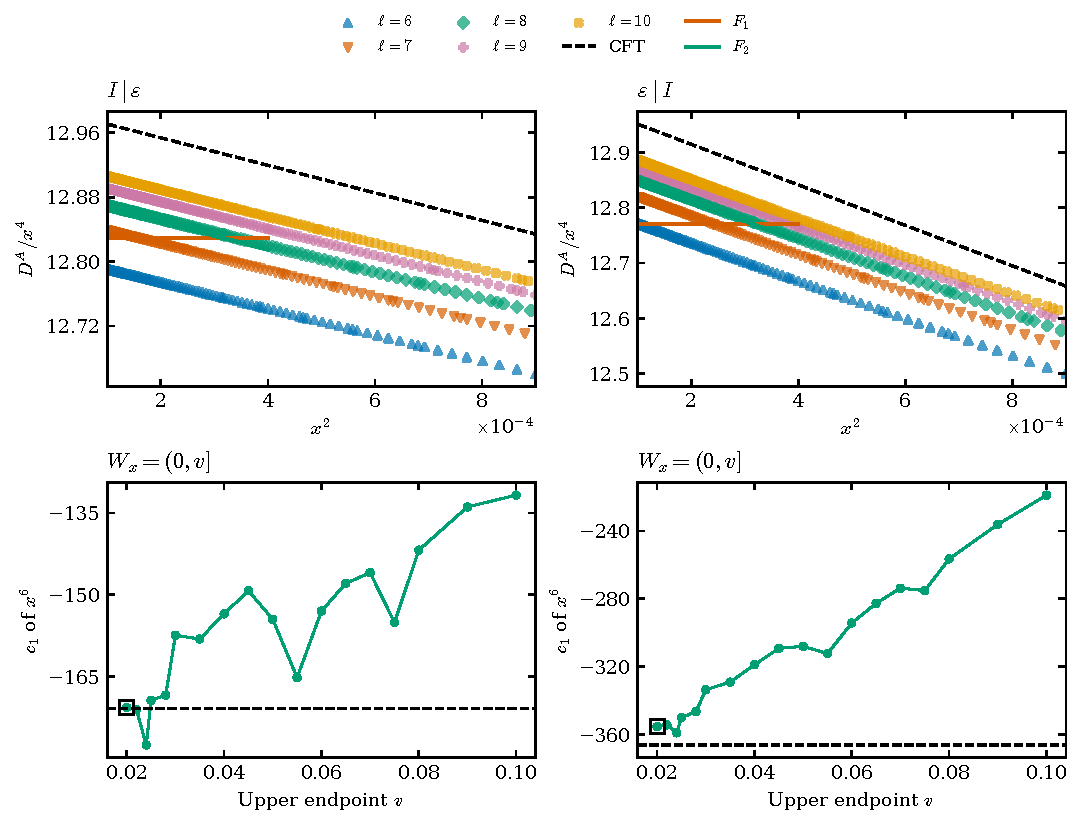
\includegraphics[width=.97\linewidth]{../figs/dense_known_ising.pdf}
\caption{Direct test of the two known Ising second-order coefficients at $p=1/2$. Top: the normalization in Eq.~\eqref{eq:dense-normalized-curve}, zoomed to $0.01\leq x\leq0.03$ with $\ell=6,\ldots,10$, to resolve the fitted slope and the offsets between lengths. The black dashed line is Eq.~\eqref{eq:dense-known-ising}; the fitted lines are drawn only on their actual windows. Bottom: the inferred $x^6$ coefficient as the upper endpoint varies while the displayed lower endpoint stays fixed. Squares mark the reported windows. $I\mid \varepsilon$: $W_x=(0,0.02]$, $m=1255$, $c_0=12.883$, $c_1=-170.71$; $\varepsilon\mid I$: $W_x=(0,0.02]$, $m=1255$, $c_0=12.882$, $c_1=-355.38$. Both $F_2$ coefficients are free; the objective is in $D^A$, not in $D^A/x^4$.}
\label{fig:dense-known}
\end{figure}

\begin{figure}[!htbp]\centering
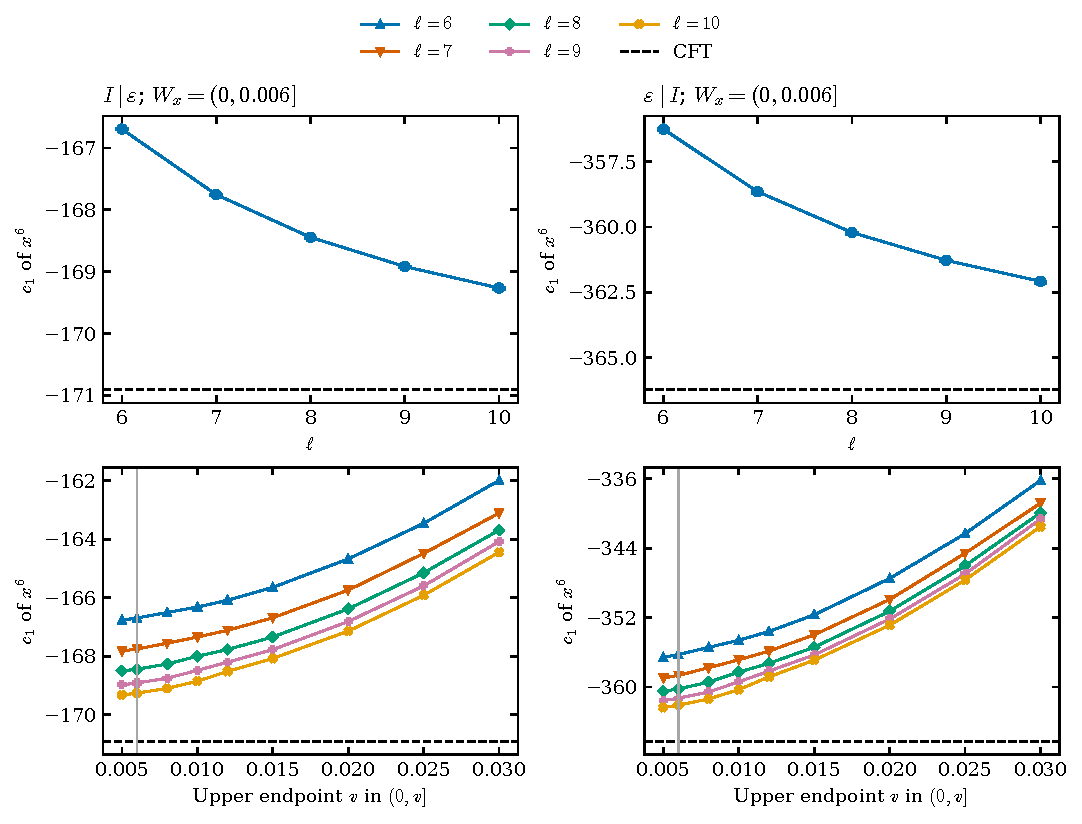
\includegraphics[width=.97\linewidth]{../figs/dense_fixed_subsystem.pdf}
\caption{The same two-power Ising fit performed separately at each subsystem length. Both $x^4$ and $x^6$ coefficients are fitted freely with their exponents fixed; no lattice-correction term is added. Top: vertical bars are the range of $c_1$ across omitted-size refits, not statistical confidence intervals; the marker is the full-data estimate. The black dashed values are Eq.~\eqref{eq:dense-known-ising}. Bottom: coefficient drift as the upper endpoint varies, with each length fitted independently; the vertical line marks the tabulated window. Every fit and every omitted-size training set contains at least forty points. Table~\ref{tab:dense-subsystem} gives the exact counts, both coefficients, and discrepancies.}
\label{fig:dense-subsystem}
\end{figure}

\begin{figure}[!htbp]\centering
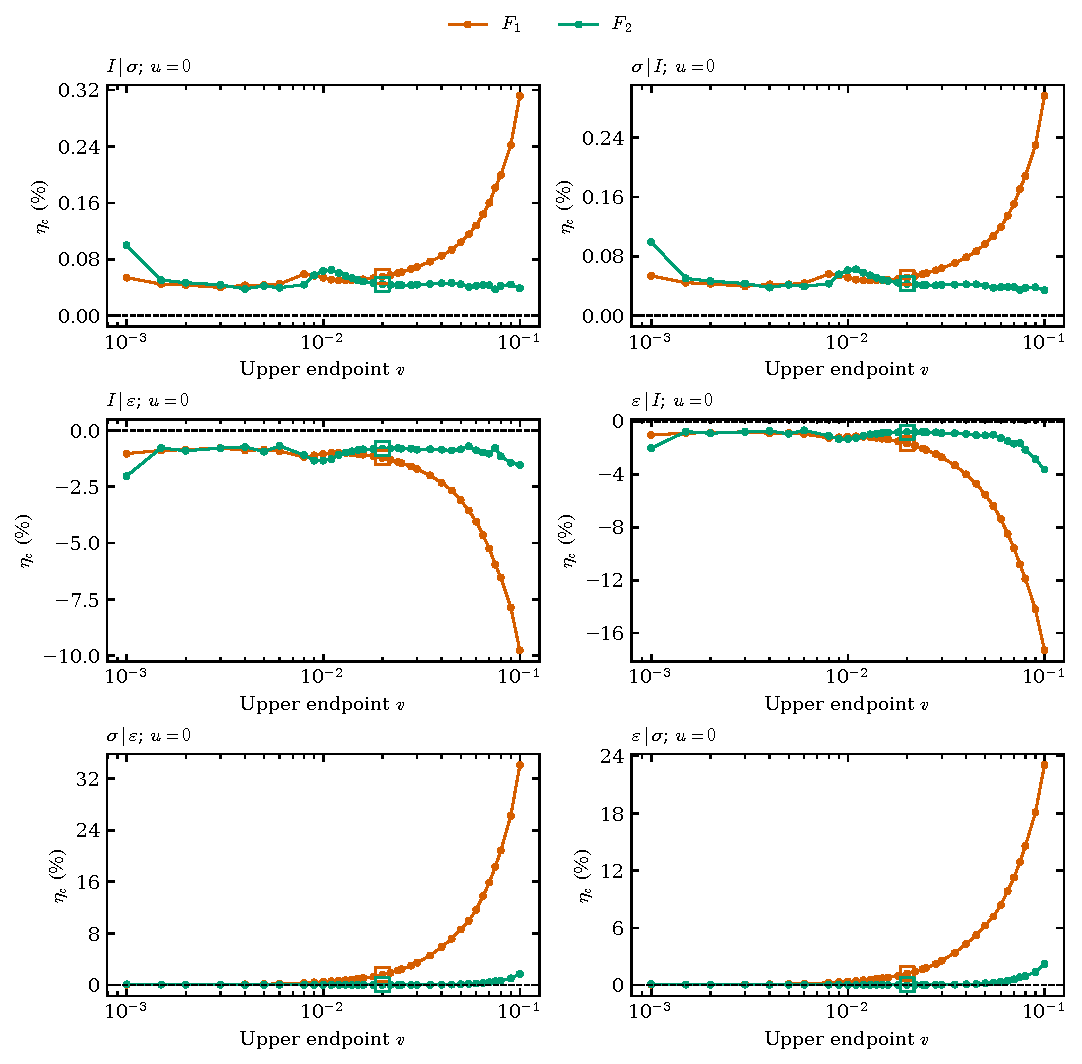
\includegraphics[width=.97\linewidth]{../figs/dense_coefficients_small_ising.pdf}
\caption{Ising small intervals: leading-coefficient discrepancy $\eta_c$ against the upper endpoint $v\leq0.1$ of $W=[u,v]$. Each panel states its fixed $u$; only windows with at least forty points in every omitted-size training set are shown. $F_1$ and $F_2$ always use identical points; $F_2$ fixes both manuscript powers. Squares mark the principal-table windows. All ordinates are linear. The zero line is the theoretical leading coefficient, with its full power of $\pi$.}
\label{fig:dense-coefficients-small-ising}
\end{figure}

\begin{figure}[!htbp]\centering
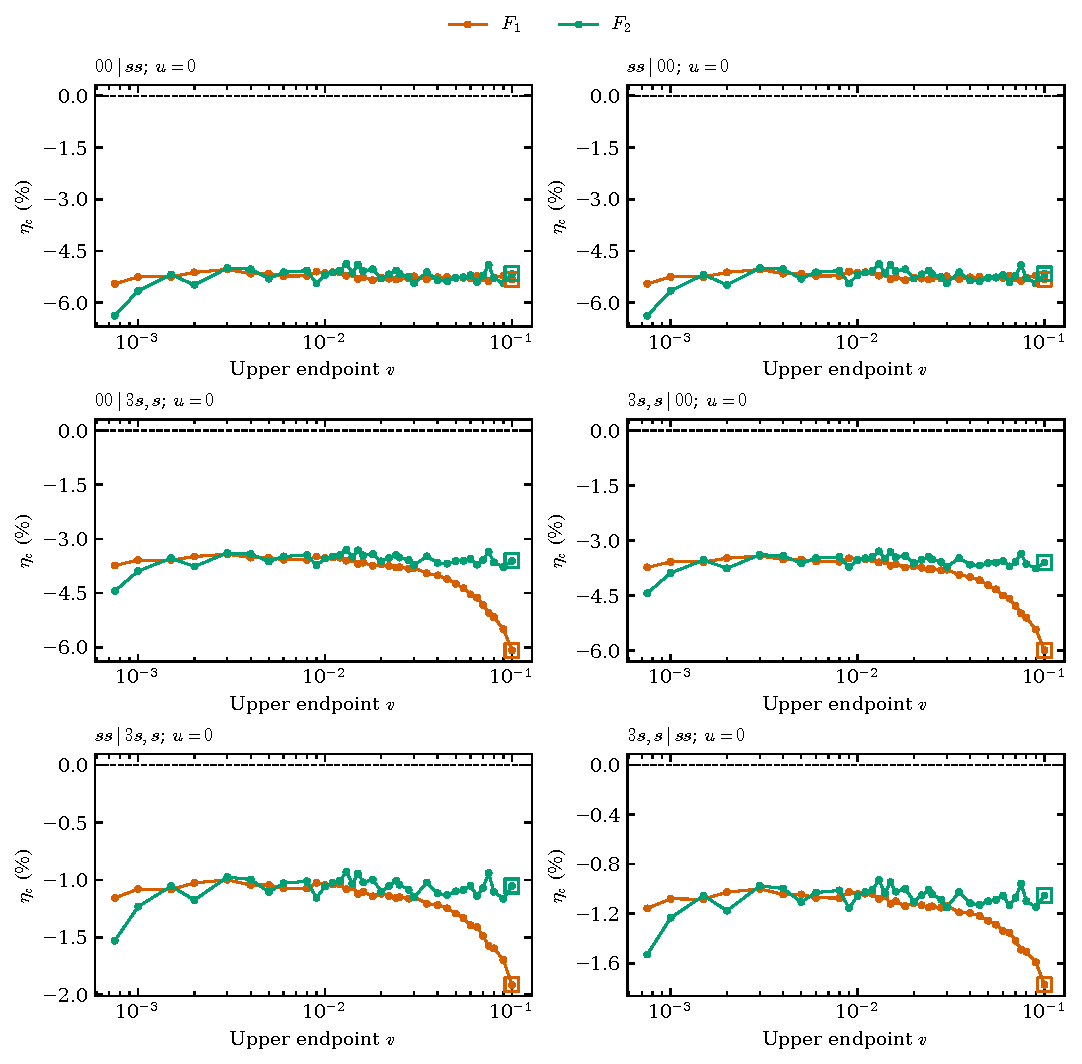
\includegraphics[width=.97\linewidth]{../figs/dense_coefficients_small_boson.pdf}
\caption{Compact boson small intervals: leading-coefficient discrepancy $\eta_c$ against the upper endpoint $v\leq0.1$ of $W=[u,v]$. Each panel states its fixed $u$; only windows with at least forty points in every omitted-size training set are shown. $F_1$ and $F_2$ always use identical points; $F_2$ fixes both manuscript powers. Squares mark the principal-table windows. All ordinates are linear. The zero line is the theoretical leading coefficient, with its full power of $\pi$.}
\label{fig:dense-coefficients-small-boson}
\end{figure}

\begin{figure}[!htbp]\centering
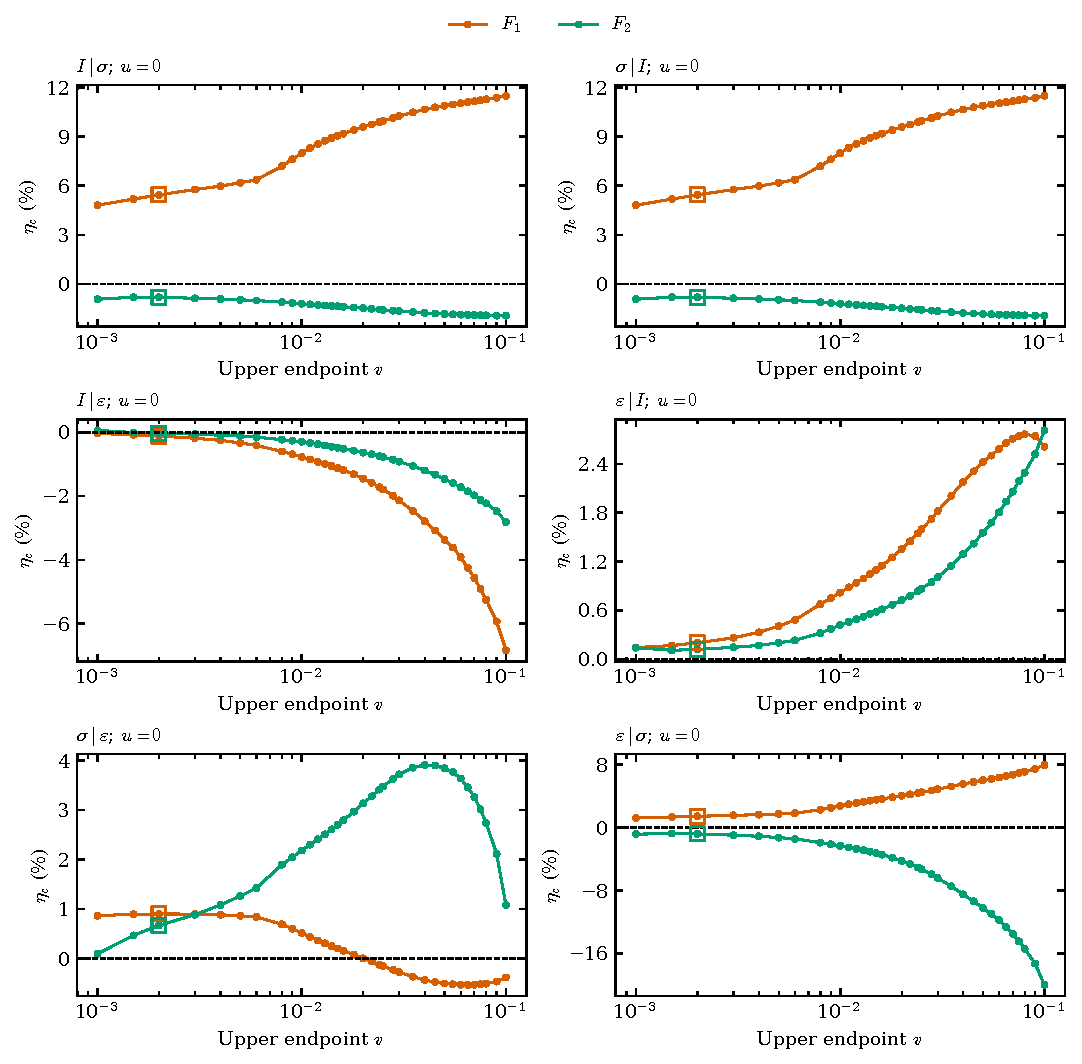
\includegraphics[width=.97\linewidth]{../figs/dense_coefficients_large_ising.pdf}
\caption{Ising large intervals: leading-coefficient discrepancy $\eta_c$ against the upper endpoint $v\leq0.1$ of $W=[u,v]$. Each panel states its fixed $u$; only windows with at least forty points in every omitted-size training set are shown. $F_1$ and $F_2$ always use identical points; $F_2$ fixes both manuscript powers. Squares mark the principal-table windows. All ordinates are linear. The zero line is the theoretical leading coefficient, with its full power of $\pi$.}
\label{fig:dense-coefficients-large-ising}
\end{figure}

\begin{figure}[!htbp]\centering
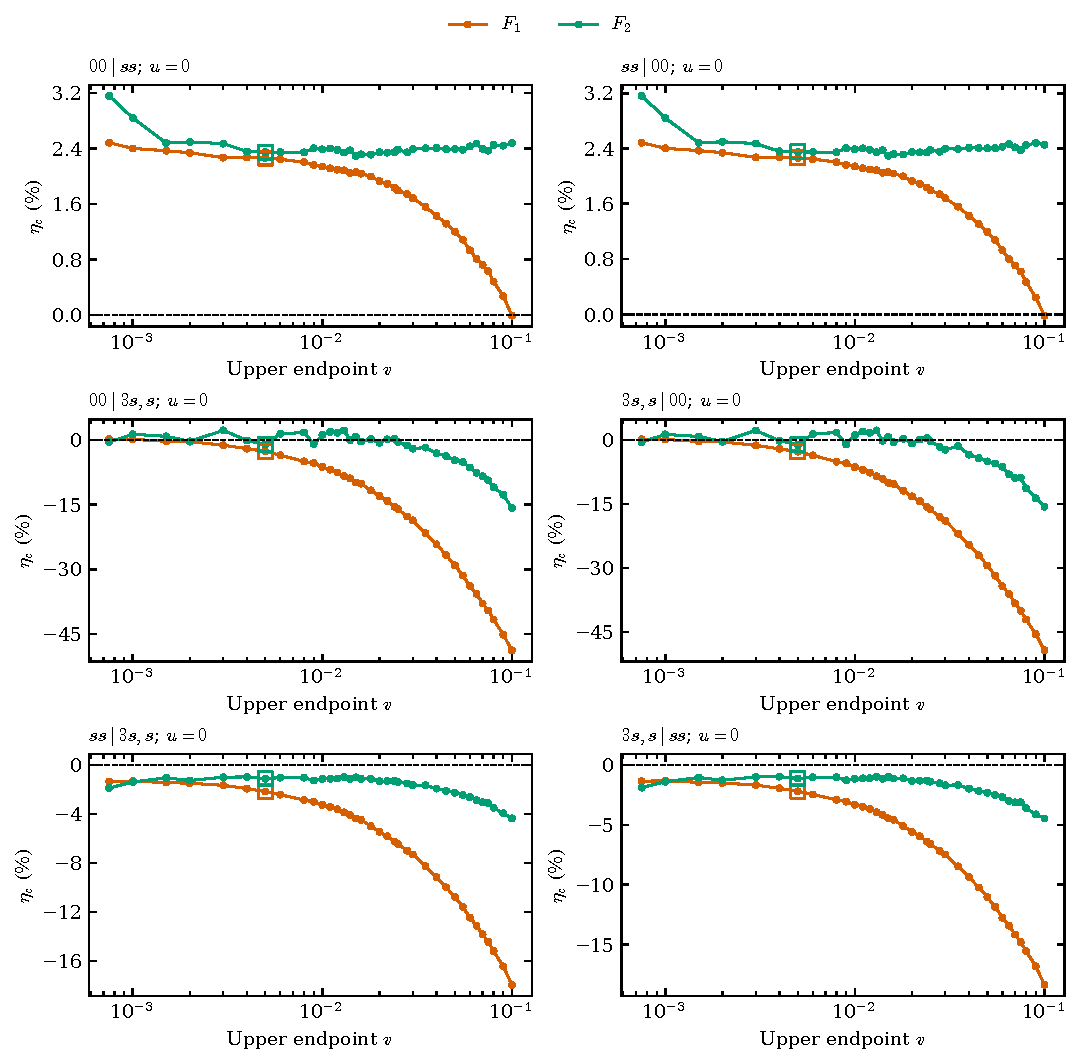
\includegraphics[width=.97\linewidth]{../figs/dense_coefficients_large_boson.pdf}
\caption{Compact boson large intervals: leading-coefficient discrepancy $\eta_c$ against the upper endpoint $v\leq0.1$ of $W=[u,v]$. Each panel states its fixed $u$; only windows with at least forty points in every omitted-size training set are shown. $F_1$ and $F_2$ always use identical points; $F_2$ fixes both manuscript powers. Squares mark the principal-table windows. All ordinates are linear. The zero line is the theoretical leading coefficient, with its full power of $\pi$.}
\label{fig:dense-coefficients-large-boson}
\end{figure}

\begin{figure}[!htbp]\centering
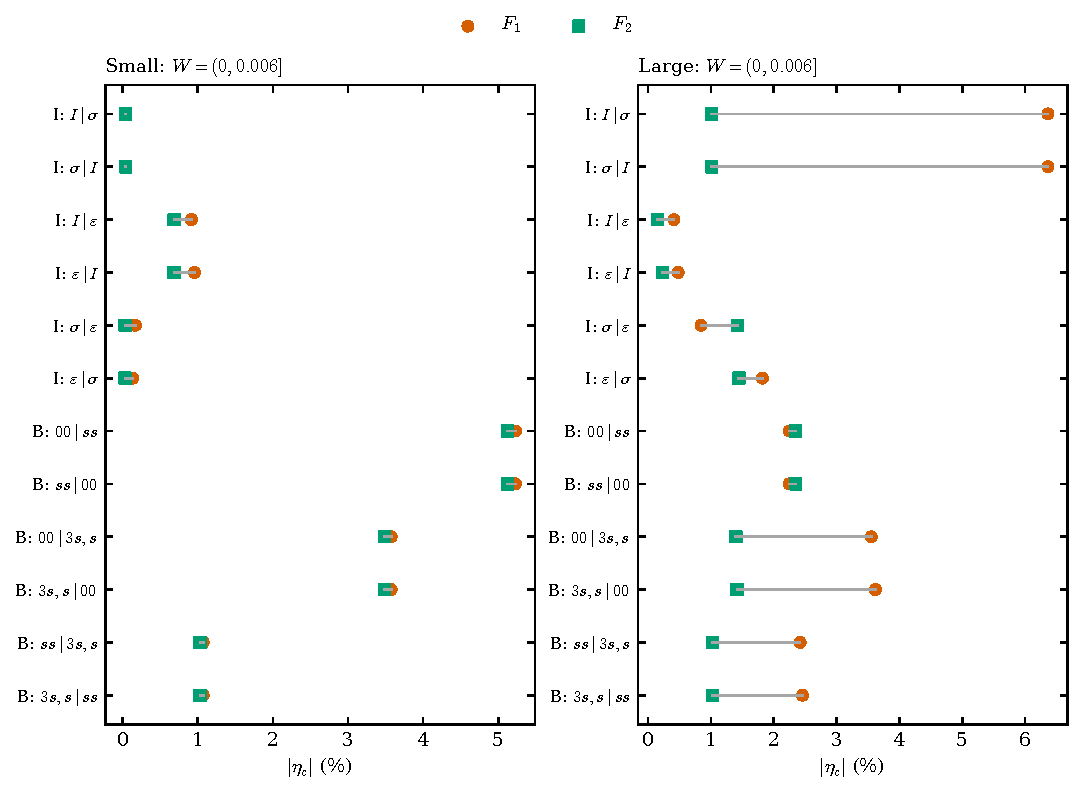
\includegraphics[width=.97\linewidth]{../figs/dense_shared_window.pdf}
\caption{A separate single-window diagnostic across all ordered pairs, using the current enlarged data and distinct from the adopted CFT-specific windows in Eq.~\eqref{eq:common-fit-windows}. I and B identify Ising and compact boson. A leftward shift from the circle ($F_1$) to the square ($F_2$) improves the leading coefficient. The same displayed interval and the same observations are used for both models; powers are fixed to the pair-specific manuscript values. Coefficients include powers of $\pi$, and $|\eta_c|$ is the absolute percentage discrepancy in Eq.~\eqref{eq:metrics}. The original largest sizes and $\ell=6,\ldots,10$ are retained.}
\label{fig:dense-shared}
\end{figure}

\subsection{Matched-window results and reproduction}
The source \path{src/conformal_blocks/dense_windows.py} regenerates
the scan and matched-window comparisons from completed CSVs.
The portable \path{fitting_datas} notebook includes per-model window
controls and the complete scan, selected comparisons, and omitted-size
records. Its defaults keep all models and directions in each CFT and
interval group on the same window. Separate-length and shared-window
figures are explicitly identified diagnostics.
\begingroup\footnotesize
\begingroup\setlength{\tabcolsep}{2pt}
\begin{longtable}{llrrrrrrrr}
\caption{Ising small intervals: identical-window coefficient comparison at $p=1/2$, $\ell=6,\ldots,10$. The displayed $W$ contains $m$ observations. $c_0$ multiplies the leading power and $c_1$ the second manuscript power; both include powers of $\pi$. The column $\Delta_0$ is Eq.~\eqref{eq:dense-coefficient-gain}, in percentage points; $G_{\rm CV}$ is the omitted-size residual gain in Eq.~\eqref{eq:cv}. Positive values mean improvement, but the two measures test different properties. Blank analytical second coefficients are unavailable. Powers and all model parameters are listed in Table~\ref{tab:ising-small-parameters}.}
\label{tab:dense-small-ising}\\\toprule
Direction & $W$ & $m$ & $c_0(F_1)$ & $c_0(F_2)$ & $c_0^{\rm CFT}$ & $c_1(F_2)$ & $c_1^{\rm CFT}$ & $\Delta_0$ & $G_{\rm CV}$\\\midrule
\endfirsthead
\toprule
Direction & $W$ & $m$ & $c_0(F_1)$ & $c_0(F_2)$ & $c_0^{\rm CFT}$ & $c_1(F_2)$ & $c_1^{\rm CFT}$ & $\Delta_0$ & $G_{\rm CV}$\\\midrule
\endhead
\bottomrule\endfoot
$I\mid \sigma$ & $(0,0.02]$ & 1255 & 0.20573 & 0.20571 & 0.20562 & 0.083833 &  & 0.010494 & 2.077\\
$\sigma\mid I$ & $(0,0.02]$ & 1255 & 0.20572 & 0.2057 & 0.20562 & 0.069099 &  & 0.0086493 & 1.8149\\
$I\mid \varepsilon$ & $(0,0.02]$ & 1255 & 12.83 & 12.883 & 12.988 & -170.71 & -170.91 & 0.41412 & 3.8386\\
$\varepsilon\mid I$ & $(0,0.02]$ & 1255 & 12.77 & 12.882 & 12.988 & -355.38 & -366.24 & 0.86214 & 15.195\\
$\sigma\mid \varepsilon$ & $(0,0.02]$ & 1255 & 0.2089 & 0.20565 & 0.20562 & 12.604 &  & 1.5777 & 95.461\\
$\varepsilon\mid \sigma$ & $(0,0.02]$ & 1255 & 0.20806 & 0.20566 & 0.20562 & 9.3133 &  & 1.1658 & 94.318\\
\end{longtable}
\endgroup

\begingroup\setlength{\tabcolsep}{3pt}
\begin{longtable}{llrrrrrr}
\caption{Ising small intervals: second-coefficient sensitivity for Table~\ref{tab:dense-small-ising}. The extrema $c_{1,\min}^{(-N)},c_{1,\max}^{(-N)}$ come from the omitted-size refits and are not confidence bounds. $\eta_1=100(c_1/c_1^{\rm CFT}-1)$ is blank when theory supplies no coefficient. The final column is $100|c_1v^{r_1-r_0}/c_0|$, the size of the fitted second term relative to the first at the window upper endpoint $v$. A fitted nonzero coefficient is not by itself proof of a continuum coefficient.}
\label{tab:dense-small-ising-second}\\\toprule
Direction & $W$ & $c_1$ & $c_1^{\rm CFT}$ & $c_{1,\min}^{(-N)}$ & $c_{1,\max}^{(-N)}$ & $\eta_1$ [\%] & Term ratio [\%]\\\midrule
\endfirsthead
\toprule
Direction & $W$ & $c_1$ & $c_1^{\rm CFT}$ & $c_{1,\min}^{(-N)}$ & $c_{1,\max}^{(-N)}$ & $\eta_1$ [\%] & Term ratio [\%]\\\midrule
\endhead
\bottomrule\endfoot
$I\mid \sigma$ & $(0,0.02]$ & 0.083833 &  & 0.076713 & 0.089011 &  & 0.016301\\
$\sigma\mid I$ & $(0,0.02]$ & 0.069099 &  & 0.063043 & 0.073541 &  & 0.013436\\
$I\mid \varepsilon$ & $(0,0.02]$ & -170.71 & -170.91 & -181.53 & -153.57 & -0.12193 & 0.53\\
$\varepsilon\mid I$ & $(0,0.02]$ & -355.38 & -366.24 & -366.12 & -338.45 & -2.9657 & 1.1035\\
$\sigma\mid \varepsilon$ & $(0,0.02]$ & 12.604 &  & 12.595 & 12.619 &  & 2.4516\\
$\varepsilon\mid \sigma$ & $(0,0.02]$ & 9.3133 &  & 9.3048 & 9.3273 &  & 1.8114\\
\end{longtable}
\endgroup

\begingroup\setlength{\tabcolsep}{2pt}
\begin{longtable}{llrrrrrrrr}
\caption{Compact boson small intervals: identical-window coefficient comparison at $p=1/2$, $\ell=6,\ldots,10$. The displayed $W$ contains $m$ observations. $c_0$ multiplies the leading power and $c_1$ the second manuscript power; both include powers of $\pi$. The column $\Delta_0$ is Eq.~\eqref{eq:dense-coefficient-gain}, in percentage points; $G_{\rm CV}$ is the omitted-size residual gain in Eq.~\eqref{eq:cv}. Positive values mean improvement, but the two measures test different properties. Blank analytical second coefficients are unavailable. Powers and all model parameters are listed in Table~\ref{tab:boson-small-parameters}.}
\label{tab:dense-small-boson}\\\toprule
Direction & $W$ & $m$ & $c_0(F_1)$ & $c_0(F_2)$ & $c_0^{\rm CFT}$ & $c_1(F_2)$ & $c_1^{\rm CFT}$ & $\Delta_0$ & $G_{\rm CV}$\\\midrule
\endfirsthead
\toprule
Direction & $W$ & $m$ & $c_0(F_1)$ & $c_0(F_2)$ & $c_0^{\rm CFT}$ & $c_1(F_2)$ & $c_1^{\rm CFT}$ & $\Delta_0$ & $G_{\rm CV}$\\\midrule
\endhead
\bottomrule\endfoot
$00\mid ss$ & $(0,0.1]$ & 598 & 0.77866 & 0.77996 & 0.82247 & -0.1917 &  & 0.15793 & -2.5678\\
$ss\mid 00$ & $(0,0.1]$ & 598 & 0.77871 & 0.77995 & 0.82247 & -0.18219 &  & 0.1501 & -2.5842\\
$00\mid 3s,s$ & $(0,0.1]$ & 598 & 3.8623 & 3.964 & 4.1123 & -15.02 &  & 2.4748 & 35.203\\
$3s,s\mid 00$ & $(0,0.1]$ & 598 & 3.8657 & 3.9643 & 4.1123 & -14.541 &  & 2.3959 & 35.866\\
$ss\mid 3s,s$ & $(0,0.1]$ & 598 & 1.6134 & 1.6276 & 1.6449 & -2.0896 &  & 0.86075 & 18.998\\
$3s,s\mid ss$ & $(0,0.1]$ & 598 & 1.6157 & 1.6276 & 1.6449 & -1.7507 &  & 0.72113 & 18.631\\
\end{longtable}
\endgroup

\begingroup\setlength{\tabcolsep}{3pt}
\begin{longtable}{llrrrrrr}
\caption{Compact boson small intervals: second-coefficient sensitivity for Table~\ref{tab:dense-small-boson}. The extrema $c_{1,\min}^{(-N)},c_{1,\max}^{(-N)}$ come from the omitted-size refits and are not confidence bounds. $\eta_1=100(c_1/c_1^{\rm CFT}-1)$ is blank when theory supplies no coefficient. The final column is $100|c_1v^{r_1-r_0}/c_0|$, the size of the fitted second term relative to the first at the window upper endpoint $v$. A fitted nonzero coefficient is not by itself proof of a continuum coefficient.}
\label{tab:dense-small-boson-second}\\\toprule
Direction & $W$ & $c_1$ & $c_1^{\rm CFT}$ & $c_{1,\min}^{(-N)}$ & $c_{1,\max}^{(-N)}$ & $\eta_1$ [\%] & Term ratio [\%]\\\midrule
\endfirsthead
\toprule
Direction & $W$ & $c_1$ & $c_1^{\rm CFT}$ & $c_{1,\min}^{(-N)}$ & $c_{1,\max}^{(-N)}$ & $\eta_1$ [\%] & Term ratio [\%]\\\midrule
\endhead
\bottomrule\endfoot
$00\mid ss$ & $(0,0.1]$ & -0.1917 &  & -0.50151 & 0.1399 &  & 0.24579\\
$ss\mid 00$ & $(0,0.1]$ & -0.18219 &  & -0.4909 & 0.14816 &  & 0.23359\\
$00\mid 3s,s$ & $(0,0.1]$ & -15.02 &  & -16.149 & -13.84 &  & 3.7891\\
$3s,s\mid 00$ & $(0,0.1]$ & -14.541 &  & -15.603 & -13.438 &  & 3.668\\
$ss\mid 3s,s$ & $(0,0.1]$ & -2.0896 &  & -2.3303 & -1.8108 &  & 1.2839\\
$3s,s\mid ss$ & $(0,0.1]$ & -1.7507 &  & -1.9474 & -1.5292 &  & 1.0756\\
\end{longtable}
\endgroup

\begingroup\setlength{\tabcolsep}{2pt}
\begin{longtable}{llrrrrrrrr}
\caption{Ising large intervals: identical-window coefficient comparison at $p=1/2$, $\ell=6,\ldots,10$. The displayed $W$ contains $m$ observations. $c_0$ multiplies the leading power and $c_1$ the second manuscript power; both include powers of $\pi$. The column $\Delta_0$ is Eq.~\eqref{eq:dense-coefficient-gain}, in percentage points; $G_{\rm CV}$ is the omitted-size residual gain in Eq.~\eqref{eq:cv}. Positive values mean improvement, but the two measures test different properties. Blank analytical second coefficients are unavailable. Powers and all model parameters are listed in Table~\ref{tab:ising-large-parameters}.}
\label{tab:dense-large-ising}\\\toprule
Direction & $W$ & $m$ & $c_0(F_1)$ & $c_0(F_2)$ & $c_0^{\rm CFT}$ & $c_1(F_2)$ & $c_1^{\rm CFT}$ & $\Delta_0$ & $G_{\rm CV}$\\\midrule
\endfirsthead
\toprule
Direction & $W$ & $m$ & $c_0(F_1)$ & $c_0(F_2)$ & $c_0^{\rm CFT}$ & $c_1(F_2)$ & $c_1^{\rm CFT}$ & $\Delta_0$ & $G_{\rm CV}$\\\midrule
\endhead
\bottomrule\endfoot
$I\mid \sigma$ & $(0,0.002]$ & 260 & 0.65339 & 0.61463 & 0.61965 & 0.20243 &  & 4.6332 & 96.863\\
$\sigma\mid I$ & $(0,0.002]$ & 260 & 0.65339 & 0.61462 & 0.61965 & 0.20245 &  & 4.6331 & 96.886\\
$I\mid \varepsilon$ & $(0,0.002]$ & 260 & 3.2861 & 3.289 & 3.2899 & -1070.2 &  & 0.090409 & 47.468\\
$\varepsilon\mid I$ & $(0,0.002]$ & 260 & 3.2964 & 3.2938 & 3.2899 & 959.21 &  & 0.081036 & 53.25\\
$\sigma\mid \varepsilon$ & $(0,0.002]$ & 260 & 0.15631 & 0.15595 & 0.15491 & 0.0018716 &  & 0.23133 & 19.238\\
$\varepsilon\mid \sigma$ & $(0,0.002]$ & 260 & 0.15712 & 0.15365 & 0.15491 & 0.018087 &  & 0.60996 & 90.498\\
\end{longtable}
\endgroup

\begingroup\setlength{\tabcolsep}{3pt}
\begin{longtable}{llrrrrrr}
\caption{Ising large intervals: second-coefficient sensitivity for Table~\ref{tab:dense-large-ising}. The extrema $c_{1,\min}^{(-N)},c_{1,\max}^{(-N)}$ come from the omitted-size refits and are not confidence bounds. $\eta_1=100(c_1/c_1^{\rm CFT}-1)$ is blank when theory supplies no coefficient. The final column is $100|c_1v^{r_1-r_0}/c_0|$, the size of the fitted second term relative to the first at the window upper endpoint $v$. A fitted nonzero coefficient is not by itself proof of a continuum coefficient.}
\label{tab:dense-large-ising-second}\\\toprule
Direction & $W$ & $c_1$ & $c_1^{\rm CFT}$ & $c_{1,\min}^{(-N)}$ & $c_{1,\max}^{(-N)}$ & $\eta_1$ [\%] & Term ratio [\%]\\\midrule
\endfirsthead
\toprule
Direction & $W$ & $c_1$ & $c_1^{\rm CFT}$ & $c_{1,\min}^{(-N)}$ & $c_{1,\max}^{(-N)}$ & $\eta_1$ [\%] & Term ratio [\%]\\\midrule
\endhead
\bottomrule\endfoot
$I\mid \sigma$ & $(0,0.002]$ & 0.20243 &  & 0.20232 & 0.20251 &  & 6.9649\\
$\sigma\mid I$ & $(0,0.002]$ & 0.20245 &  & 0.20234 & 0.20253 &  & 6.9657\\
$I\mid \varepsilon$ & $(0,0.002]$ & -1070.2 &  & -1095.7 & -1053.3 &  & 0.13015\\
$\varepsilon\mid I$ & $(0,0.002]$ & 959.21 &  & 944.43 & 976.81 &  & 0.11649\\
$\sigma\mid \varepsilon$ & $(0,0.002]$ & 0.0018716 &  & 0.0018486 & 0.0019195 &  & 0.25379\\
$\varepsilon\mid \sigma$ & $(0,0.002]$ & 0.018087 &  & 0.018053 & 0.01811 &  & 2.4894\\
\end{longtable}
\endgroup

\begingroup\setlength{\tabcolsep}{2pt}
\begin{longtable}{llrrrrrrrr}
\caption{Compact boson large intervals: identical-window coefficient comparison at $p=1/2$, $\ell=6,\ldots,10$. The displayed $W$ contains $m$ observations. $c_0$ multiplies the leading power and $c_1$ the second manuscript power; both include powers of $\pi$. The column $\Delta_0$ is Eq.~\eqref{eq:dense-coefficient-gain}, in percentage points; $G_{\rm CV}$ is the omitted-size residual gain in Eq.~\eqref{eq:cv}. Positive values mean improvement, but the two measures test different properties. Blank analytical second coefficients are unavailable. Powers and all model parameters are listed in Table~\ref{tab:boson-large-parameters}.}
\label{tab:dense-large-boson}\\\toprule
Direction & $W$ & $m$ & $c_0(F_1)$ & $c_0(F_2)$ & $c_0^{\rm CFT}$ & $c_1(F_2)$ & $c_1^{\rm CFT}$ & $\Delta_0$ & $G_{\rm CV}$\\\midrule
\endfirsthead
\toprule
Direction & $W$ & $m$ & $c_0(F_1)$ & $c_0(F_2)$ & $c_0^{\rm CFT}$ & $c_1(F_2)$ & $c_1^{\rm CFT}$ & $\Delta_0$ & $G_{\rm CV}$\\\midrule
\endhead
\bottomrule\endfoot
$00\mid ss$ & $(0,0.005]$ & 317 & 1.2616 & 1.2627 & 1.2337 & -0.33376 &  & -0.085416 & -0.80584\\
$ss\mid 00$ & $(0,0.005]$ & 317 & 1.2616 & 1.2627 & 1.2337 & -0.34138 &  & -0.087364 & -0.7901\\
$00\mid 3s,s$ & $(0,0.005]$ & 317 & 73.093 & 74.307 & 75.109 & -265.58 &  & 1.6153 & -0.40053\\
$3s,s\mid 00$ & $(0,0.005]$ & 317 & 73.058 & 74.252 & 75.109 & -261.18 &  & 1.5885 & -0.47282\\
$ss\mid 3s,s$ & $(0,0.005]$ & 317 & 3.2185 & 3.2529 & 3.2899 & -8.6617 &  & 1.0449 & 13.931\\
$3s,s\mid ss$ & $(0,0.005]$ & 317 & 3.2176 & 3.2528 & 3.2899 & -8.8758 &  & 1.0707 & 13.775\\
\end{longtable}
\endgroup

\begingroup\setlength{\tabcolsep}{3pt}
\begin{longtable}{llrrrrrr}
\caption{Compact boson large intervals: second-coefficient sensitivity for Table~\ref{tab:dense-large-boson}. The extrema $c_{1,\min}^{(-N)},c_{1,\max}^{(-N)}$ come from the omitted-size refits and are not confidence bounds. $\eta_1=100(c_1/c_1^{\rm CFT}-1)$ is blank when theory supplies no coefficient. The final column is $100|c_1v^{r_1-r_0}/c_0|$, the size of the fitted second term relative to the first at the window upper endpoint $v$. A fitted nonzero coefficient is not by itself proof of a continuum coefficient.}
\label{tab:dense-large-boson-second}\\\toprule
Direction & $W$ & $c_1$ & $c_1^{\rm CFT}$ & $c_{1,\min}^{(-N)}$ & $c_{1,\max}^{(-N)}$ & $\eta_1$ [\%] & Term ratio [\%]\\\midrule
\endfirsthead
\toprule
Direction & $W$ & $c_1$ & $c_1^{\rm CFT}$ & $c_{1,\min}^{(-N)}$ & $c_{1,\max}^{(-N)}$ & $\eta_1$ [\%] & Term ratio [\%]\\\midrule
\endhead
\bottomrule\endfoot
$00\mid ss$ & $(0,0.005]$ & -0.33376 &  & -0.53362 & -0.14815 &  & 0.13216\\
$ss\mid 00$ & $(0,0.005]$ & -0.34138 &  & -0.53762 & -0.15672 &  & 0.13518\\
$00\mid 3s,s$ & $(0,0.005]$ & -265.58 &  & -373.74 & -178.05 &  & 1.7871\\
$3s,s\mid 00$ & $(0,0.005]$ & -261.18 &  & -372.89 & -175.63 &  & 1.7588\\
$ss\mid 3s,s$ & $(0,0.005]$ & -8.6617 &  & -9.6333 & -8.0378 &  & 1.3314\\
$3s,s\mid ss$ & $(0,0.005]$ & -8.8758 &  & -9.8805 & -8.2283 &  & 1.3643\\
\end{longtable}
\endgroup

\begingroup\setlength{\tabcolsep}{3pt}
\begin{longtable}{lrrrrrrr}
\caption{Known Ising coefficient checks separated by subsystem length, at $p=1/2$ and the common window $W_x=(0,0.006]$. Each row fits $c_0x^4+c_1x^6$ to the stated $\ell$ only; $m$ counts distinct chain sizes. The theoretical coefficients are Eq.~\eqref{eq:dense-known-ising}; $\eta_j=100(c_j/c_j^{\rm CFT}-1)$, $j=0,1$, are signed percentage discrepancies. The final column gives the extrema from omitting each chain size and refitting. These deterministic ranges are sensitivity measures, not confidence intervals.}
\label{tab:dense-subsystem}\\\toprule
Direction & $\ell$ & $m$ & $c_0$ & $\eta_0$ [\%] & $c_1$ & $\eta_1$ [\%] & $c_1$ omitted-size range\\\midrule
\endfirsthead
\toprule
Direction & $\ell$ & $m$ & $c_0$ & $\eta_0$ [\%] & $c_1$ & $\eta_1$ [\%] & $c_1$ omitted-size range\\\midrule
\endhead
\bottomrule\endfoot
$I\mid \varepsilon$ & 6 & 97 & 12.808 & -1.3871 & -166.69 & -2.4684 & $[-166.71,-166.69]$\\
$I\mid \varepsilon$ & 7 & 92 & 12.855 & -1.0194 & -167.75 & -1.8482 & $[-167.77,-167.75]$\\
$I\mid \varepsilon$ & 8 & 89 & 12.886 & -0.78063 & -168.45 & -1.4442 & $[-168.47,-168.44]$\\
$I\mid \varepsilon$ & 9 & 86 & 12.908 & -0.61689 & -168.92 & -1.1677 & $[-168.93,-168.92]$\\
$I\mid \varepsilon$ & 10 & 82 & 12.923 & -0.49974 & -169.27 & -0.96408 & $[-169.28,-169.26]$\\
$\varepsilon\mid I$ & 6 & 97 & 12.808 & -1.3872 & -356.25 & -2.7295 & $[-356.3,-356.24]$\\
$\varepsilon\mid I$ & 7 & 92 & 12.855 & -1.0194 & -358.64 & -2.075 & $[-358.73,-358.64]$\\
$\varepsilon\mid I$ & 8 & 89 & 12.886 & -0.78069 & -360.21 & -1.6477 & $[-360.3,-360.2]$\\
$\varepsilon\mid I$ & 9 & 86 & 12.908 & -0.61696 & -361.28 & -1.3561 & $[-361.32,-361.27]$\\
$\varepsilon\mid I$ & 10 & 82 & 12.923 & -0.4998 & -362.08 & -1.1357 & $[-362.16,-362.08]$\\
\end{longtable}
\endgroup

\endgroup

\clearpage
\subsection{Zero-anchored common windows on the denser data}
\label{sec:common-window-results}
The small-Ising and small-boson windows remain $(0,0.02]$ and
$(0,0.1]$. The large-interval comparison adopts $(0,0.002]$ for Ising
and the prescribed $(0,0.005]$ for the compact boson. These are the
four windows of Eq.~\eqref{eq:common-fit-windows}; every model and
all six directions within each group use identical observations.
The preceding data refinement added 48 even system sizes for each CFT, with all five
lengths $\ell=6,7,8,9,10$ at each size. The largest sizes remain
$8192$ and $16384$. Every added geometry enters the corresponding
small-interval window; only those satisfying the separate large-interval
cutoff enter its fits. Both observables are computed and preserved.
The data refinement initially kept all four windows fixed. A subsequent
zero-anchored search selected the historical large-boson cutoff $0.0047$.
The current revision changes that cutoff to the prescribed $0.005$,
on exactly the same raw data. All theoretical powers are unchanged.
At the current cutoff, $F_2$ improves four of the six large-boson
leading coefficients; the all-six target is not met.

The new sizes are chosen using geometry alone. For each CFT, seed
the even sizes at which each length first enters its large-interval
window. Repeatedly bisect the largest gap in $\log N$, choosing the
nearest unused even size to the geometric midpoint. Add 32 sizes
in $3000\leq N\leq8192$ for Ising or $3750\leq N\leq16384$ for
the boson. Add 16 further sizes in $500\leq N\leq3000$ or
$100\leq N\leq3750$, respectively. Existing sizes are never
recomputed or replaced. The exact executed lists are included in
Eq.~\eqref{eq:extended-grid} and the data manifest below.

Table~\ref{tab:common-window-counts} gives the updated counts. On the adopted windows, $F_2$ improves the absolute leading-coefficient discrepancy in 22 of 24 cases and omitted-size prediction in 18 of 24 cases. All models use the same observations within each group. The current large-boson cutoff is prescribed as $0.005$; the earlier coefficient-guided choice $0.0047$ is retained as a historical comparison.

The added sizes pass all 10512 stored production checks of the types in Table~\ref{tab:scaling-numerical-checks}. Recomputing 450 directed rows from saved matrices reproduces every recorded value exactly. No entropy calculation or physical observation is changed by this window revision.

The two small-interval windows and all their coefficients are unchanged from the denser-data revision. The known Ising $x^6$ coefficients and their discrepancies are given in Tables~\ref{tab:dense-small-ising} and \ref{tab:dense-small-ising-second}.

\begingroup\footnotesize
\begingroup\setlength{\tabcolsep}{3pt}
\begin{longtable}{lllrrrrr}
\caption{Adopted common-window results for $p=1/2$, $\ell=6,\ldots,10$. Counts apply to every direction. The last two columns count directions with positive leading-coefficient gain $\Delta_0$ in Eq.~\eqref{eq:dense-coefficient-gain} and positive omitted-size prediction gain $G_{\rm CV}$ in Eq.~\eqref{eq:cv}, respectively. All three fitted models use the stated window. The large-boson upper cutoff is prescribed as $0.005$.}
\label{tab:common-window-counts}\\\toprule
Interval & CFT & $W$ & $m$ & Sizes & Min. training & $\Delta_0>0$ & $G_{\rm CV}>0$\\\midrule
\endfirsthead
\toprule
Interval & CFT & $W$ & $m$ & Sizes & Min. training & $\Delta_0>0$ & $G_{\rm CV}>0$\\\midrule
\endhead
\bottomrule\endfoot
small & ising & $(0,0.02]$ & 1255 & 278 & 1250 & 6/6 & 6/6\\
small & boson & $(0,0.1]$ & 598 & 124 & 593 & 6/6 & 4/6\\
large & ising & $(0,0.002]$ & 260 & 67 & 255 & 6/6 & 6/6\\
large & boson & $(0,0.005]$ & 317 & 68 & 312 & 4/6 & 2/6\\
\end{longtable}
\endgroup

\endgroup

For large Ising, the adopted window retains 260 observations per direction at 67 distinct chain sizes. Relative to $F_1$ on those observations, $F_2$ improves the leading coefficient in 6 of six directions and omitted-size prediction in 6 of six. The coefficient gain stays positive in every omitted-size refit for 6 directions. Table~\ref{tab:common-large-ising} compares with the preceding report window on the same numerical grid.

\begingroup\footnotesize
\begingroup\setlength{\tabcolsep}{3pt}
\begin{longtable}{lrrrrr}
\caption{Ising large intervals: absolute leading-coefficient discrepancies $E_0=|\eta_c|$, with $\eta_c$ defined in Eq.~\eqref{eq:metrics}. Both versions use the same numerical grid. The previous $F_2$ column uses $(0,0.002]$ with 260 observations per direction; the current fits use $(0,0.002]$ with 260. $G_{\rm CV}$ compares $F_2$ with $F_1$ on the same current window and observations. The last column counts omitted-size refits in which $\Delta_0>0$. All discrepancies and gains are percentages; these are deterministic comparisons, not statistical error bars.}
\label{tab:common-large-ising}\\\toprule
Direction & $E_0(F_1)$ & $E_0(F_2)$ & Previous $E_0(F_2)$ & $G_{\rm CV}$ & Positive folds\\\midrule
\endfirsthead
\toprule
Direction & $E_0(F_1)$ & $E_0(F_2)$ & Previous $E_0(F_2)$ & $G_{\rm CV}$ & Positive folds\\\midrule
\endhead
\bottomrule\endfoot
$I\mid \sigma$ & 5.4442 & 0.81098 & 0.81098 & 96.863 & 67/67\\
$\sigma\mid I$ & 5.4445 & 0.81139 & 0.81139 & 96.886 & 67/67\\
$I\mid \varepsilon$ & 0.11533 & 0.024918 & 0.024918 & 47.468 & 67/67\\
$\varepsilon\mid I$ & 0.19921 & 0.11818 & 0.11818 & 53.25 & 67/67\\
$\sigma\mid \varepsilon$ & 0.9017 & 0.67037 & 0.67037 & 19.238 & 67/67\\
$\varepsilon\mid \sigma$ & 1.4228 & 0.81285 & 0.81285 & 90.498 & 67/67\\
\end{longtable}
\endgroup

\endgroup

For large compact boson, the adopted window retains 317 observations per direction at 68 distinct chain sizes. Relative to $F_1$ on those observations, $F_2$ improves the leading coefficient in 4 of six directions and omitted-size prediction in 2 of six. The coefficient gain stays positive in every omitted-size refit for 4 directions. Table~\ref{tab:common-large-boson} compares with the preceding report window on the same numerical grid.

$00\mid ss$ has absolute leading discrepancies $2.2645\%$ under $F_1$ and $2.34992\%$ under $F_2$. Its omitted-size prediction gain is $-0.805838\%$, and the leading gain stays positive in 0 of 68 refits. Negative prediction gains denote worse prediction.

$ss\mid 00$ has absolute leading discrepancies $2.26363\%$ under $F_1$ and $2.351\%$ under $F_2$. Its omitted-size prediction gain is $-0.790097\%$, and the leading gain stays positive in 0 of 68 refits. Negative prediction gains denote worse prediction.

$00\mid 3s,s$ has absolute leading discrepancies $2.68291\%$ under $F_1$ and $1.06764\%$ under $F_2$. Its omitted-size prediction gain is $-0.400526\%$, and the leading gain stays positive in 68 of 68 refits. Negative prediction gains denote worse prediction.

$3s,s\mid 00$ has absolute leading discrepancies $2.72951\%$ under $F_1$ and $1.14099\%$ under $F_2$. Its omitted-size prediction gain is $-0.47282\%$, and the leading gain stays positive in 68 of 68 refits. Negative prediction gains denote worse prediction.

\begingroup\footnotesize
\begingroup\setlength{\tabcolsep}{3pt}
\begin{longtable}{lrrrrr}
\caption{Compact boson large intervals: absolute leading-coefficient discrepancies $E_0=|\eta_c|$, with $\eta_c$ defined in Eq.~\eqref{eq:metrics}. Both versions use the same numerical grid. The previous $F_2$ column uses $(0,0.0047]$ with 311 observations per direction; the current fits use $(0,0.005]$ with 317. $G_{\rm CV}$ compares $F_2$ with $F_1$ on the same current window and observations. The last column counts omitted-size refits in which $\Delta_0>0$. All discrepancies and gains are percentages; these are deterministic comparisons, not statistical error bars.}
\label{tab:common-large-boson}\\\toprule
Direction & $E_0(F_1)$ & $E_0(F_2)$ & Previous $E_0(F_2)$ & $G_{\rm CV}$ & Positive folds\\\midrule
\endfirsthead
\toprule
Direction & $E_0(F_1)$ & $E_0(F_2)$ & Previous $E_0(F_2)$ & $G_{\rm CV}$ & Positive folds\\\midrule
\endhead
\bottomrule\endfoot
$00\mid ss$ & 2.2645 & 2.3499 & 2.2855 & -0.80584 & 0/68\\
$ss\mid 00$ & 2.2636 & 2.351 & 2.2855 & -0.7901 & 0/68\\
$00\mid 3s,s$ & 2.6829 & 1.0676 & 2.197 & -0.40053 & 68/68\\
$3s,s\mid 00$ & 2.7295 & 1.141 & 2.2251 & -0.47282 & 68/68\\
$ss\mid 3s,s$ & 2.1683 & 1.1234 & 0.8515 & 13.931 & 68/68\\
$3s,s\mid ss$ & 2.1982 & 1.1274 & 0.84555 & 13.775 & 68/68\\
\end{longtable}
\endgroup

\clearpage
\begingroup\setlength{\tabcolsep}{4pt}
\begin{longtable}{lrrrrr}
\caption{Concrete neighboring-cutoff tests for the large intervals. Every row uses $W_y=(0,v]$ for all directions, both fitted powers fixed as in Table~\ref{tab:complement-theory}, and $\ell=6,\ldots,10$. The two count columns use the definitions in Table~\ref{tab:common-window-counts}. The last column is the largest absolute leading-coefficient discrepancy among the six $F_2$ fits, in percent. The changing $m$ shows when a cutoff adds an actual observation.}
\label{tab:common-window-neighbors}\\\toprule
CFT & $v$ & $m$ & $\Delta_0>0$ & $G_{\rm CV}>0$ & Max. $E_0(F_2)$\\\midrule
\endfirsthead
\toprule
CFT & $v$ & $m$ & $\Delta_0>0$ & $G_{\rm CV}>0$ & Max. $E_0(F_2)$\\\midrule
\endhead
\bottomrule\endfoot
ising & 0.0015 & 175 & 6/6 & 6/6 & 0.80928\\
ising & 0.002 & 260 & 6/6 & 6/6 & 0.81285\\
ising & 0.0025 & 314 & 6/6 & 6/6 & 0.90129\\
ising & 0.003 & 348 & 6/6 & 5/6 & 0.97471\\
ising & 0.004 & 389 & 5/6 & 6/6 & 1.1168\\
boson & 0.0016 & 193 & 2/6 & 2/6 & 2.4537\\
boson & 0.0045 & 308 & 4/6 & 4/6 & 2.3172\\
boson & 0.0046 & 308 & 4/6 & 4/6 & 2.3172\\
boson & 0.00465 & 310 & 4/6 & 4/6 & 2.3126\\
boson & 0.00469 & 310 & 4/6 & 4/6 & 2.3126\\
boson & 0.0047 & 311 & 6/6 & 4/6 & 2.2855\\
boson & 0.00472 & 311 & 6/6 & 4/6 & 2.2855\\
boson & 0.00474 & 311 & 6/6 & 4/6 & 2.2855\\
boson & 0.00475 & 312 & 4/6 & 4/6 & 2.2959\\
boson & 0.0048 & 313 & 4/6 & 2/6 & 2.3298\\
boson & 0.0049 & 315 & 4/6 & 2/6 & 2.3732\\
boson & 0.005 & 317 & 4/6 & 2/6 & 2.351\\
\end{longtable}
\endgroup

\endgroup

The zero-anchored search on the current grid enumerates every distinct selection $W_y=(0,v]$ through $v=0.20$, requiring at least forty observations after omitting any chain size. It contains 1361 admissible Ising windows and 532 boson windows. Of the Ising windows, 258 improve all six leading estimates and 251 also improve omitted-size prediction in all six directions. The already adopted Ising cutoff remains suitable.

For the boson, exactly one distinct data selection improves all six leading estimates. The corresponding upper cutoffs satisfy \begin{equation}0.004691689008042895\leq v<0.004741833508956797.\label{eq:zero-equivalent-cutoffs}\end{equation} The rounded value $v=0.0047$ lies in this range. The existing endpoint comparison tolerance is $10^{-14}$. There are no observations between the bounding fractions, so changing $v$ inside this range does not provide a new sampling test.

Table~\ref{tab:common-window-neighbors} retains the neighboring failures. The historical all-six coefficient gain at $0.0047$ disappears at the immediately adjacent selections; its weakest gain, for $ss\mid00$, is only about $0.00555$ percentage points. No enumerated zero-anchored boson window improves both coefficient accuracy and omitted-size prediction in all six directions. Figures~\ref{fig:zero-anchored-scan} and \ref{fig:zero-anchored-zoom} show this cutoff dependence. The currently prescribed window $0<y\leq0.005$ has 317 observations per direction and improves 4 of six leading coefficients; it does not meet the all-six target.

The earlier exhaustive search on 23472 observations and the subsequent fixed-window density comparison remain historical records. Their windows and conclusions must not be substituted for this search on the enlarged grid. All physical data are preserved; only derived selection flags and fitted summaries change in this revision.

\begin{sloppypar}The current directed results are in \path{data/common_cft_coefficient_comparison.csv}; \path{data/zero_adoption_cv.csv} and \path{data/zero_neighbor_cv.csv} retain the omitted-size fits. Files prefixed \texttt{zero\_anchored\_} contain the exhaustive scan and its validation; files prefixed \texttt{zero\_before\_} preserve the preceding report. The portable \path{fitting_datas} notebook uses the same adopted windows and refitted coefficients. The two cutoff figures have linear discrepancy ordinates.\end{sloppypar}

\clearpage
\begin{figure}[p]
\centering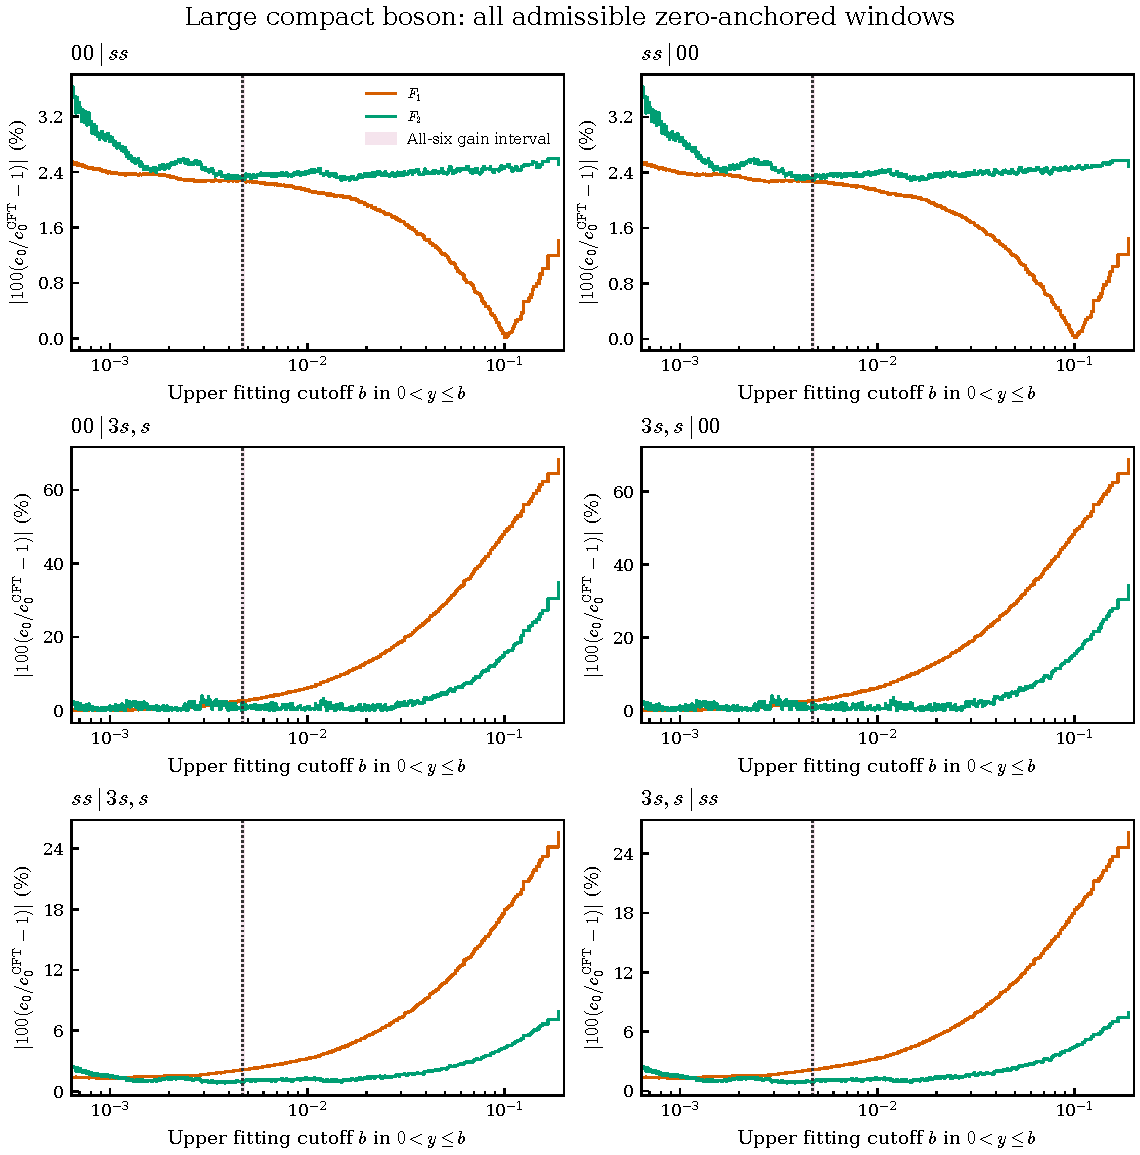
\includegraphics[width=\textwidth,height=.83\textheight,keepaspectratio]{../figs/zero_anchored_cutoff_scan.pdf}
\caption{Large-boson leading-coefficient accuracy across all admissible zero-anchored windows $W_y=(0,v]$ through $v=0.20$, using $p=1/2$ and $\ell=6,7,8,9,10$. The plotting symbol $b$ on the horizontal axis denotes the trial upper cutoff $v$, not a primary-state label. Each step corresponds to a distinct selected data set with at least forty training observations after any chain-size omission. Both powers of $F_2$ are fixed to Table~\ref{tab:complement-theory}; $F_1$ uses only its leading power. The ordinate is $|\eta_c|$ from Eq.~\eqref{eq:metrics}, on a linear scale. The dotted line marks the previous candidate $v=0.0047$, and the shaded band marks Eq.~\eqref{eq:zero-equivalent-cutoffs}. The current prescribed cutoff is $0.005$; its counts and minimum training sizes are in Table~\ref{tab:common-window-counts}.}
\label{fig:zero-anchored-scan}
\end{figure}
\clearpage
\begin{figure}[p]
\centering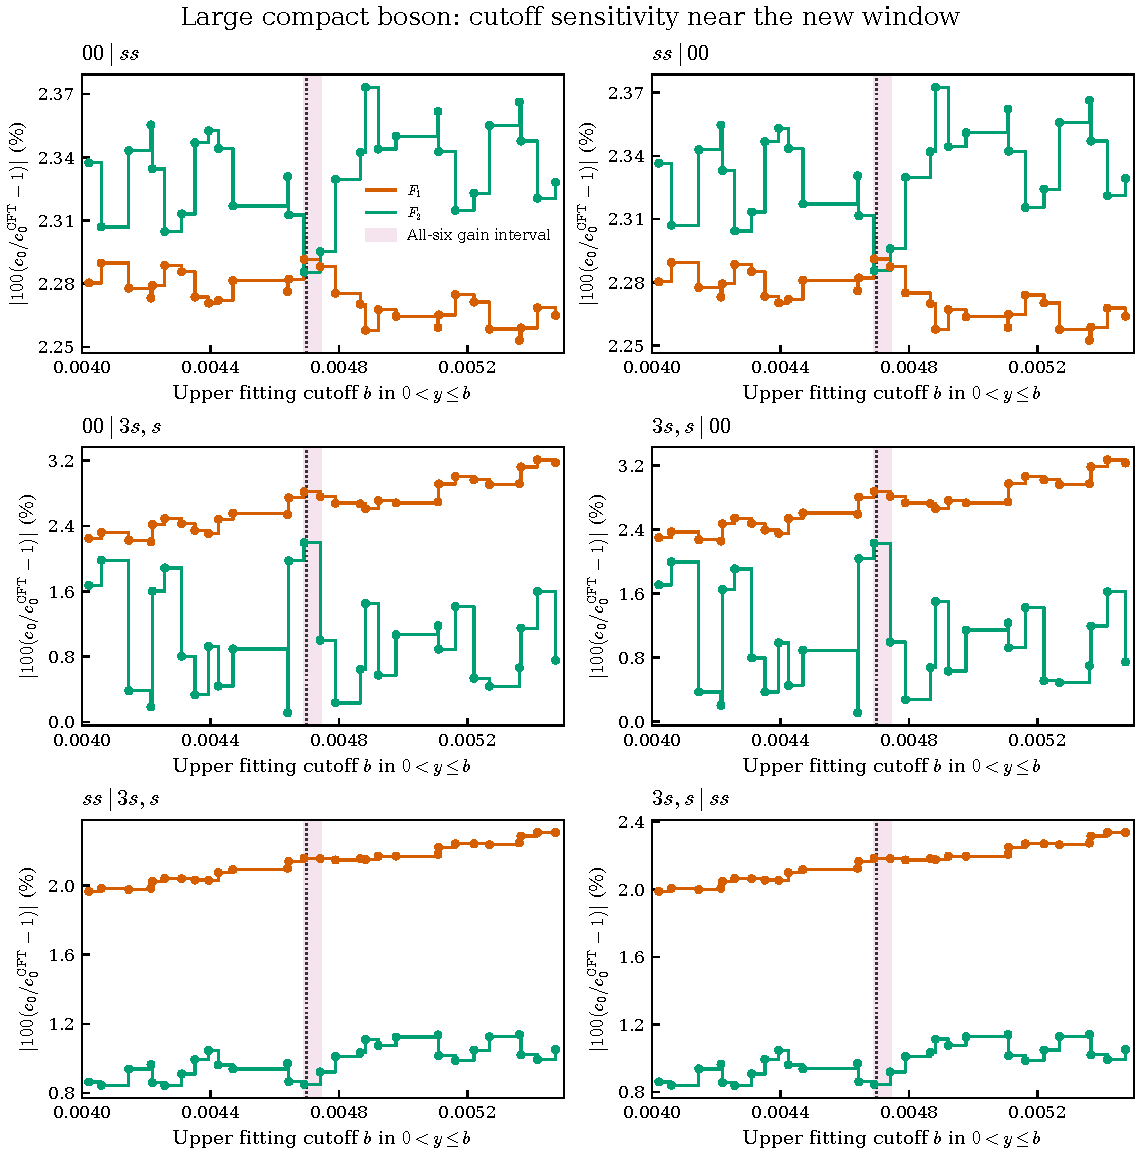
\includegraphics[width=\textwidth,height=.83\textheight,keepaspectratio]{../figs/zero_anchored_cutoff_zoom.pdf}
\caption{Historical cutoff sensitivity around the previous large-boson candidate $0.0047$, using the same data, models and discrepancy as Fig.~\ref{fig:zero-anchored-scan}. Markers show actual changes of data membership; both axes are linear. The shaded historical interval has 311 points per direction from 68 chain sizes. The nearest selections outside it lose the all-six leading-coefficient gain, as quantified in Table~\ref{tab:common-window-neighbors}. The residual reduction alone does not establish coefficient recovery.}
\label{fig:zero-anchored-zoom}
\end{figure}
\clearpage


